\section{Вычислительные эксперименты}
\subsection{Цель и проверяемые свойства}
Цель базового эксперимента --- сравнить ошибку и профили решений
маршрутизаторов при фиксированных экспертах, доступных признаках
и одинаковой квоте эскалаций. Проверяется зависимость от количества
парных примеров обучения и бюджета второго вызова. Прирост каскада
над первой моделью, разница между правилами при одной квоте и обмен
спасений на вред рассматриваются как разные результаты.

\subsection{Данные и разбиение}
Используется BANKING77: англоязычные банковские обращения с 77
намерениями \citep{review17}. Источник --- PolyAI revision
\texttt{57ec275d8078af65b7731c2a98be812d844a6d6b}, лицензия CC BY 4.0.
Из 10\,003 train-строк удалены четыре нормализованных повтора;
9\,999 строк стратифицированно разделены на expert-train 5\,999,
calibration 1\,000, router-fit 2\,000 и policy-dev 1\,000.
Нормализация для аудита --- NFKC, нижний регистр и свёртка пробелов.
Между train-частями текстовых пересечений нет. Official test 3\,080
сохранён; дополнительная оценка без семи train/test пересечений и
одного test-повтора содержит 3\,072 строки. Manifest фиксирует
исходные индексы, SHA и seeds разбиения 20260922, 20260923, 20260924.
Часть calibration используется для аудита экспертов, не для настройки роутера.

\subsection{Фиксированные эксперты}
В базовой конфигурации используются две пары: TF--IDF+LR с BERT-tiny
и TF--IDF+LR с frozen MiniLM+LR. Все эксперты обучаются только
на expert-train. Внутреннее разбиение 80/20 служит для выбора параметров,
после чего выполняется refit на всех 5\,999 строках.

TF--IDF использует word n-grams (1,2), min\_df=2, sublinear TF
и ограничение 30\,000 признаков. LR настраивается по
$C\in\{0.25,1,4,16\}$; выбран $C=16$.
Frozen MiniLM --- \texttt{sentence-transformers/all-MiniLM-L6-v2},
revision \texttt{1110a243fdf4706b3f48f1d95db1a4f5529b4d41}:
нормализованный mean pooling и LR,
$C\in\{0.25,1,4,16,64\}$, выбран $C=64$.
BERT-tiny --- \texttt{prajjwal1/bert-tiny}, revision
\texttt{6f75de8b60a9f8a2fdf7b69cbd86d9e64bcb3837};
mean pooling и линейная классификационная голова.
Во внутренней валидации выбраны восемь эпох; refit выполнен с AdamW,
batch 32, encoder LR $10^{-4}$, head LR $10^{-3}$,
weight decay 0.01, warmup/linear decay и gradient norm cap 1.
Максимальная длина --- 64 токена, seed обучения --- 20261002.

Accuracy на official test: TF--IDF 86.56\%, BERT-tiny 84.71\%,
frozen MiniLM 92.31\%. Направления исходных пар заданы измеренной
стоимостью вызова, а не точностью: более дорогой эксперт может быть
хуже в среднем. Прогнозы экспертов зафиксированы до обучения роутеров.

\subsection{Признаки, методы и настройка}
Восемь признаков: максимальная вероятность, top-two margin,
нормированная энтропия, сумма квадратов вероятностей, вторая и третья
вероятности и log1p длины запроса в символах/словах. Ответ и признаки
второй модели недоступны при решении. Правильность и эталон используются
как supervision и для оценки, не как входные признаки.

Сравниваются confidence (низкая максимальная вероятность), logistic
weak-error, ridge direct на $D$ и две logistic rescue/harm-головы
со score $\widehat p_+-\widehat p_-$. Weak-error вычитает из
предсказанной ошибки первой модели среднюю train-ошибку второй;
это proxy, а не точная условная сравнительная полезность.
В каждом условии методы используют одинаковые fit/dev строки,
признаки и tie-breaking keys. Классы функций и число параметров
различаются; сравнение не является строго capacity-matched.

Объёмы fit --- 200/500/1\,000, dev=fit/2;
10 seeds подвыборок 0--9, квоты 10/20/40\%.
Подвыборки без возвращения вложены по размеру; scaler оценивается
только на выбранном fit. L2-grid --- $\{0.001,0.01,0.1,1\}$;
выбор --- по dev MSE, при точном равенстве выбирается более сильная
регуляризация. Для ridge $\alpha=n\lambda$, для logistic
$C=(n\lambda)^{-1}$; intercept не штрафуется.
Train/dev/test роутера сохраняют естественное распределение.
Бюджет данных включает настройку: 300/750/1\,500 использованных пар.

Вычисляются accuracy, observed-$D$ MSE, числа спасений и вредных замен,
таблица $Z_r$ и разброс по обучениям. Для каждого пакета выбираются
ровно $\lfloor bN\rfloor$ запросов; при 20\% это 616 вызовов
из 3\,080. Квота не является измеренной экономией денег или
end-to-end latency. Базовая сетка содержит 60 условий и 180
финальных обучаемых роутеров; с четырьмя правилами, тремя квотами
и двумя версиями test получается 1\,440 строк метрик.

\subsection{Результаты}
\begin{table}[htbp]\centering
\caption{TF--IDF $\to$ frozen MiniLM, fit 1\,000/dev 500,
20\% эскалаций. Средние и SD по 10 подвыборкам.}\label{tab:base}
\begin{tabular}{lrr}
\toprule
Способ & Accuracy, \% & SD, п.п. \\
\midrule
confidence & 90{,}68 & 0{,}00 \\
weak\_error & 91{,}27 & 0{,}07 \\
direct & 91{,}48 & 0{,}23 \\
events & 91{,}53 & 0{,}17 \\
\bottomrule
\end{tabular}

\end{table}
\begin{figure}[htbp]\centering
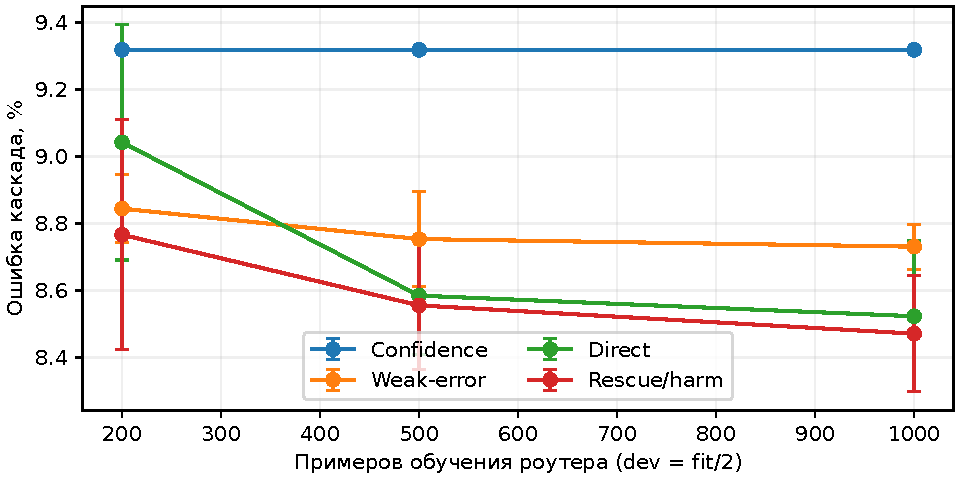
\includegraphics[width=.82\linewidth]{figures/error_curve.pdf}
\caption{Ошибка каскада при изменении fit и dev=fit/2,
TF--IDF $\to$ frozen MiniLM, 20\% вызовов. Полосы --- SD по
10 подвыборкам обучения.}\label{fig:error}
\end{figure}

Результаты представлены в таблице~\ref{tab:base} и на
рисунке~\ref{fig:error}. При увеличении обучения ошибка части
правил снижается; SD по подвыборкам не является доверительным
интервалом из независимых задач. При fit 1\,000 direct и events
имеют близкие средние accuracy, поэтому различия в сотых процента
не рассматриваются как практическое преимущество.

На рисунке~\ref{fig:profiles} показан описательный пример другой пары.
Confidence исправляет в среднем 123 ответа и портит 102,
Events --- 85.2 и 51.1. Таким образом, меняется профиль решений:
снижаются и спасения, и вредные замены. Пример выбран после
просмотра пилота; отдельный статистический тест компонентов пока
не проведён. Более широкий post-hoc анализ accuracy с общей поправкой
на множественность не установил убедительного превосходства
правил в проверенном режиме. Отсутствие значимости не означает
практическую эквивалентность.

\begin{figure}[htbp]\centering
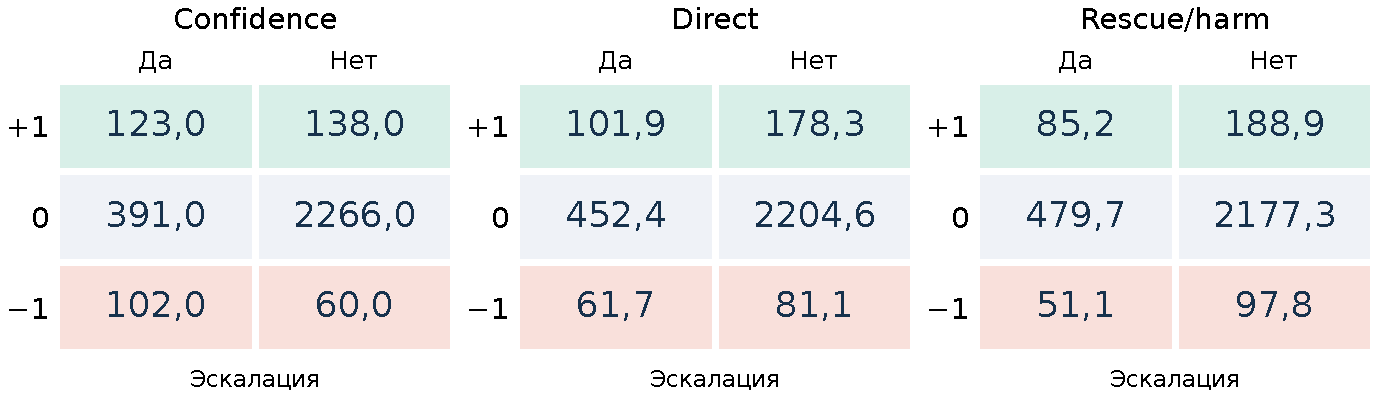
\includegraphics[width=\linewidth]{figures/decision_profiles.pdf}
\caption{TF--IDF $\to$ BERT-tiny, fit 1\,000/dev 500,
20\% вызовов, средние counts по 10 обучениям. Строки ---
выигрыш выбранного действия относительно противоположного;
колонки --- эскалация да/нет.}\label{fig:profiles}
\end{figure}

\subsection{Воспроизводимость}
Исходники и данные:
\url{https://github.com/Nastik05/Cost-sensitive-routing}.
Команда \texttt{python3 code/run.py} заново обучает роутеры по
фиксированному кэшу, проверяет 1\,440 строк метрик против исходного
прогона и генерирует рисунки/таблицу. Это повтор обучения роутеров,
а не независимое переобучение экспертов или новый test.
Параметры экспертов, source revisions и хеши сохранены в
\texttt{code/data/manifest.json}. Вычисления и визуализация разделены;
численные фрагменты текста строятся из результатов автоматически.
